% use paper, or submit
% use 11 pt (preferred), 12 pt, or 10 pt only

\documentclass[letterpaper, preprint, paper,11pt]{AAS}	% for preprint proceedings
%\documentclass[letterpaper, paper,11pt]{AAS}		% for final proceedings (20-page limit)
%\documentclass[letterpaper, paper,12pt]{AAS}		% for final proceedings (20-page limit)
%\documentclass[letterpaper, paper,10pt]{AAS}		% for final proceedings (20-page limit)
%\documentclass[letterpaper, submit]{AAS}			% to submit to JAS

\usepackage{bm}
\usepackage{amsmath}
\usepackage{subfigure}
%\usepackage[notref,notcite]{showkeys}  % use this to temporarily show labels
\usepackage[colorlinks=true, pdfstartview=FitV, linkcolor=black, citecolor= black, urlcolor= black]{hyperref}
\usepackage{overcite}
\usepackage{footnpag}			      	% make footnote symbols restart on each page

% Added packages 2019 Feb 17
\usepackage{float}
\usepackage{amssymb}
\usepackage{mathrsfs} 
%\usepackage{graphicx} % Allows including images
%\usepackage{mathrsfs}
\usepackage{booktabs} % Allows the use of \toprule, \midrule and \bottomrule in tables
\usepackage{multicol}



\PaperNumber{19-801}



\begin{document}
	
	\title{SUN-AVOIDANCE SLEW PLANNING ALGORITHM WITH POINTING AND ACTUATOR CONSTRAINTS}
	
	\author{
		Mohammad Ayoubi\thanks{Associate Professor, Department of Mechanical Engineering, Santa Clara University, 500 El Camino Real, Santa Clara, CA 95053 U.S.A. AIAA senior member, AAS senior member.} and Junette Hsin\thanks{Engineer, Dynamics and Control Analysis Group, Maxar Space Solutions (formerly Space Systems/Loral), 3825 Fabian Way, Palo Alto, CA 94303 U.S.A.}
	}
	
	
	\maketitle{} 		
	
	
	\begin{abstract}
		
		This paper presents a geometric approach for a sun (or any bright object) avoidance slew maneuver with pointing and actuator constraints. We assume spacecraft has a single light-sensitive payload with control-torque and reaction wheels' angular momentum constraints. Furthermore, we assume the initial and final attitudes, instrument boresight vector, and sun vector are known. Then we use Pontryagin's minimum principle (PMP) and derive the desired or target-frame quaternions, angular velocity and acceleration. In the end, a Monte Carlo simulation is performed to show the viability of the proposed algorithm with control-torque and angular momentum constraints. 
		% for two cases: 1) with control-torque and reaction wheels' angular momentum constraints, and 2) with control-torque. constraint.  		
	\end{abstract}

%%%%%%%%%%%%

	\section{Numerical simulation} 
	The proposed algorithm was examined by running cases in which the initial, final, and sun position vectors were randomized. Consider a spacecraft as a rigid body with one sensitive instrument. The orientation of the boresight of the instrument to the spacecraft body axes, the current and final (desired) positions with respect to the inertial frame, and the location of the sun vector are known. Only one exclusion zone around a bright object (the sun) is considered. The initial and final positions are outside of the exclusion zone.  
	
	\subsection{SAS Algorithm Pseudocode}
	
	\begin{enumerate}
		
		\item Find: sequence of slew maneuvers to avoid sun vector 
		
		\begin{enumerate}
			
			% SUN VECTOR INTRUSION 
			\item Check the sun vector intrusion 
			
			\begin{enumerate}
				\item Find eigenaxis $
				\hat{e}=\frac{\hat{P}_i\times\hat{P}_f}{|\hat{P}_i\times \hat{P}_f|}
				$
				\item Compute $
				\alpha=\frac{\pi}{2}-\cos^{-1}(\hat{S}\cdot_\mathcal{N}\hat{e})
				$
				\item IF $|\alpha|<\epsilon_p$, THEN find 
				$
				\vec{S}_{||}=\hat{S}\cos\alpha
				$
			\end{enumerate}
			
			% SLEW AROUND EIGENAXIS 
			\item Compute $\phi_1$:
			$
			\phi_1 = \cos^{-1}(\hat{P}_i\cdot_\mathcal{G}\hat{S}_{||})-\epsilon_p
			$
			
			% SLEW AROUND SUN VECTOR 
			\item Compute $\phi_2$:
			
			\begin{enumerate}
				\item IF $\alpha \neq 0$, THEN
				$
				\phi_2 = 2\sin^{-1}\Big( \frac{ \sin\epsilon_p}{\sin \theta}\Big),\ \theta=\cos^{-1}(\hat{P}_1\cdot\hat{S})
				$
				
				\item IF $\alpha = 0$, THEN
				$
				\phi_2 = \pi
				$
				
			\end{enumerate}
			
			% SLEW AROUND EIGENAXIS AGAIN 
			\item Compute $\phi_3$:
			$
			\phi_3 = \cos^{-1}(_\mathcal{G}\hat{P}_f.\hat{P}_2)
			$
			
		\end{enumerate}
		
		\item Find: commanded angular velocity, angular acceleration, and quaternion profiles 
		
		\begin{enumerate}
			
			\item Compute $\phi_{t} = \frac{\dot{\phi}_{max}^2}{\ddot{\phi}_{max}}$
			
			\item Compute $t_1$, $t_2$, and $t_f$. 
			
			IF $\phi > \phi_{t}$, THEN : 
			
			$
			t_1 = t_0 + \frac{\dot{\phi}_{max} - \dot{\phi}_0}{\ddot{\phi}_{max}}
			$ 
			
			$
			t_2 = t_1 + \frac{1}{\dot{\phi}_max} \big[ \phi_f - \dot{\phi}_0 (t_1 - t_0) - \frac{1}{2} \ddot{\phi}_{max} (t_f1 - t_0)^2 - \\ \frac{\dot{\phi}_{max} ( \dot{\phi}_{max} -  \dot{\phi}_f ) }{\ddot{\phi}_{max}} + \frac{ (\dot{\phi}_{max} - \dot{\phi}_f)^2}{2 \ddot{\phi}_{max}} \big]
			$
			
			$
			t_f=t_1+\frac{1}{\dot{\phi}_{max}}\Big[ \phi_f-\dot{\phi}_0(t_1-t_0)-\frac{1}{2}\ddot{\phi}_{max}(t_1-t_0)^2+\frac{(\dot{\phi}_{max}-\dot{\phi}_f)^2}{2\ddot{\phi}_{max}} \Big].
			$
			
			ELSE: 
			
			$ t_f = \sqrt{\frac{\dot{\phi}_{max}^2}{\ddot{\phi}_{max}}}
			$
			
			$ t_2 = t_f / 2 $ 
			
			$ t_1 = t_2 $ 
			
			\item Find ${}^DR^N$: 
			$
			{}^DR^N = \big[(cos\phi)I_{3x3} + (1 - cos\phi)\hat{e}\hat{e}^T - (sin\alpha)E^x \big]
			$
			
			\item Find $_\mathcal{B}\dot{\omega}^{D}$: 
			$
			_\mathcal{B}\dot{\omega}^{D} = {}^DR^N \ddot{\phi}_{max} \cdot _\mathcal{N}\hat{e}
			$
			
			\item Solve for control torque, $u$: 
			$
			J \cdot _\mathcal{B}\dot{\omega}^D = u - _\mathcal{B}\omega^C \times J \cdot _\mathcal{B}\omega^C 
			$
			
			\item FOR each $\phi$ between switching times, propagate $\omega$ and $q$ between switching times by solving above eqn and 
			$
			\dot{q} = \frac{1}{2} \Omega q 
			$
			
			where
			\[ \Omega = \left[ \begin{array}{cccc}
			0 & \omega_3 & -\omega_2 & \omega_1 \\
			-\omega_3 & 0 & -\omega_1 & \omega_2 \\
			\omega_2 & -\omega_1 & 0 & \omega_3 \\ 
			-\omega_1 & \omega_2 & -\omega_3 & 0 \\ 
			\end{array} \right] \] 
			
			with correct $u$ for each switching time interval. 
			
		\end{enumerate} 
	\end{enumerate}
	
%	The progression of the spacecraft along its orbit was not incorporated in these simulations, therefore, the sun vector does not change during the slew maneuvers. However, the orbit must be taken into account in real missions, thus the location of the sun vector during the $\phi_2$ portion of the maneuvers should be considered. Or rather, the timing of the instrument boresight overlapping with the sun vector projection onto the slew plane should be used in the calculation of the slew angles. 
	
	The results show that the angular velocity and acceleration never exceed the velocity and acceleration constraints for any axis. There is no noise modeled in the actuator system, as the purpose of this simulation was to validate the slewing maneuvers described by the algorithm.
	
	The attitude and rates were computed within each switching time interval for a constant control torque. For example, in the case of $\phi_2$ for the interval from $t_0$ to $t_1$, the torque in the inertial frame was found from $\tau = J \ddot{\phi}_{max}$, where $J$ is the inertia of the SC in the body frame, and $\ddot{\phi}_{max}$ is the desired (maximum) acceleration in the body frame. However, $\ddot{\phi}_{max}$ needs to go the sun vector $_\mathcal{N}S$, which is fixed in the inertial frame. To find $\ddot{\phi}_{max}$, the rotation from the inertial to (desired) body frame needed to be calculated, which is possible from $ {}^DR^N = \big[(cos\phi)I_{3x3} + (1 - cos\phi)\hat{e}\hat{e}^T - (sin\alpha)E^x \big] $. 
	
	With the desired direction of acceleration known, the necessary control torque can be solved for from Euler's equations for rigid body dynamics $	J \cdot _\mathcal{B}\dot{\omega}^D = u - _\mathcal{B}\omega^C \times J \cdot _\mathcal{B}\omega^C	$. Though real spacecraft have multiple bodies and flexible appendages, the spacecraft was assumed to be a rigid body for algorithm demonstration purposes. Once $u$ is solved, the propagation of $\omega$ and $q$ was performed by discretely solving the dynamical and kinematic equations of motion with a simulation rate of 100 Hz. The process was repeated for the interval from $t_1$ to $t_2$, except the torque applied was 0. For $t_2$ to $t_f$, the acceleration applied was $-\ddot{\phi}_{max}$, as the spacecraft needed to slew down to reach its final point for that leg of the slew. 
	
	Two cases are shown here - one in which the sun angle is greater than 0 from the slew plane. The other case is one in which the sun vector lies directly on the slew plane, so that $\phi_2 = 180$ degrees. 
		
	\subsection{Case I: $\alpha > 0$} 
		
		The parameters for a test case in which the sun vector did not lie directly on the slew plane are shown in Table \ref{tab:alphaNot0_PiPfS_AWmax}. The calculated slew angles are shown in Table \ref{tab:alphaNot0_phi_123}. 
		
		The constraints for maximum angular velocity and acceleration were chosen to demonstrate that the angular velocity and acceleration profiles would follow the switching times if-else statements, should the $\phi$ exceed the angle threshold $\phi_{t}$. The spacecraft slews from the initial to the target position during the maneuvers, and $P_1$ and $P_2$ are connected via a rotation around the sun vector. This is found to be true no matter the sun vector's position relative to the slew plane. 
		
		
		
		\begin{multicols}{2}
			\begin{table}[H]
				\centering
				\caption{Initial, Final, and Sun Positions in Inertial Frame and Constraints (Sample Inputs)}
				\begin{tabular}{lc}
					\toprule
					\midrule
					Unit Vector & Comp \\
					\midrule
					$P_i$ & [-0.50, 0.57, 0.65] \\
					$P_f$ & [0.76, -0.48, -0.44] \\ 
					$S$ & [0.30, -0.50, -0.81] \\
					\midrule
					\midrule
					Parameter & Constraint \\ 
					\midrule
					$\alpha_{max}$ & 1 $rad/s^2$ \\
					$\omega_{max}$ & 1 $rad/s$ \\ 
					\midrule
					\bottomrule
				\end{tabular}%
				\label{tab:alphaNot0_PiPfS_AWmax}%
			\end{table}
			\columnbreak
			\begin{table}[H]
				\centering
				\caption{Slew Angles $\phi_1$, $\phi_2$, and $\phi_3$}
				\begin{tabular}{lc}
					\toprule
					\midrule
					$\phi$ & deg \\
					\midrule
					1 & 32.08 \\
					2 & 102.56 \\ 
					3 & 17.76 \\
					\midrule
					\bottomrule
				\end{tabular}%
				\label{tab:alphaNot0_phi_123}%
			\end{table}%
		\end{multicols}
		
%			\begin{figure}[H]
%			\begin{center}
%				\label{fig:phi2_geometry}
%				\includegraphics[width=4.75in]{figures/alphaNot0/chord_geometry_phi2.png}
%				\caption{Chord geometry for finding $\phi_2$.}
%			\end{center}
%			\end{figure}
		
%		For the first phase of the slew, the spacecraft was rotated around the eigenaxis of the slew plane by $\phi_1$. For the second phase of the slew, the spacecraft was rotated around the sun vector fixed in inertial space by $\phi_2$. For the third phase of the slew, the spacecraft was rotated around the eigenaxis of the slew plane by $\phi_3$. The attitude generated would look like the profile in Figure \ref{fig:phi1_phi2_phi3}. 	
			
			\begin{figure}[H]
				\begin{center}
					\includegraphics[width=4.75in]{figures/alphaNot0/phi1_phi2_phi3.png}
					\caption{Attitude Profile of the Entire Slew.}
					\label{fig:phi1_phi2_phi3}
				\end{center}		
			\end{figure}	
		
	\begin{multicols}{2}
		\begin{figure}[H]
			\begin{center}
			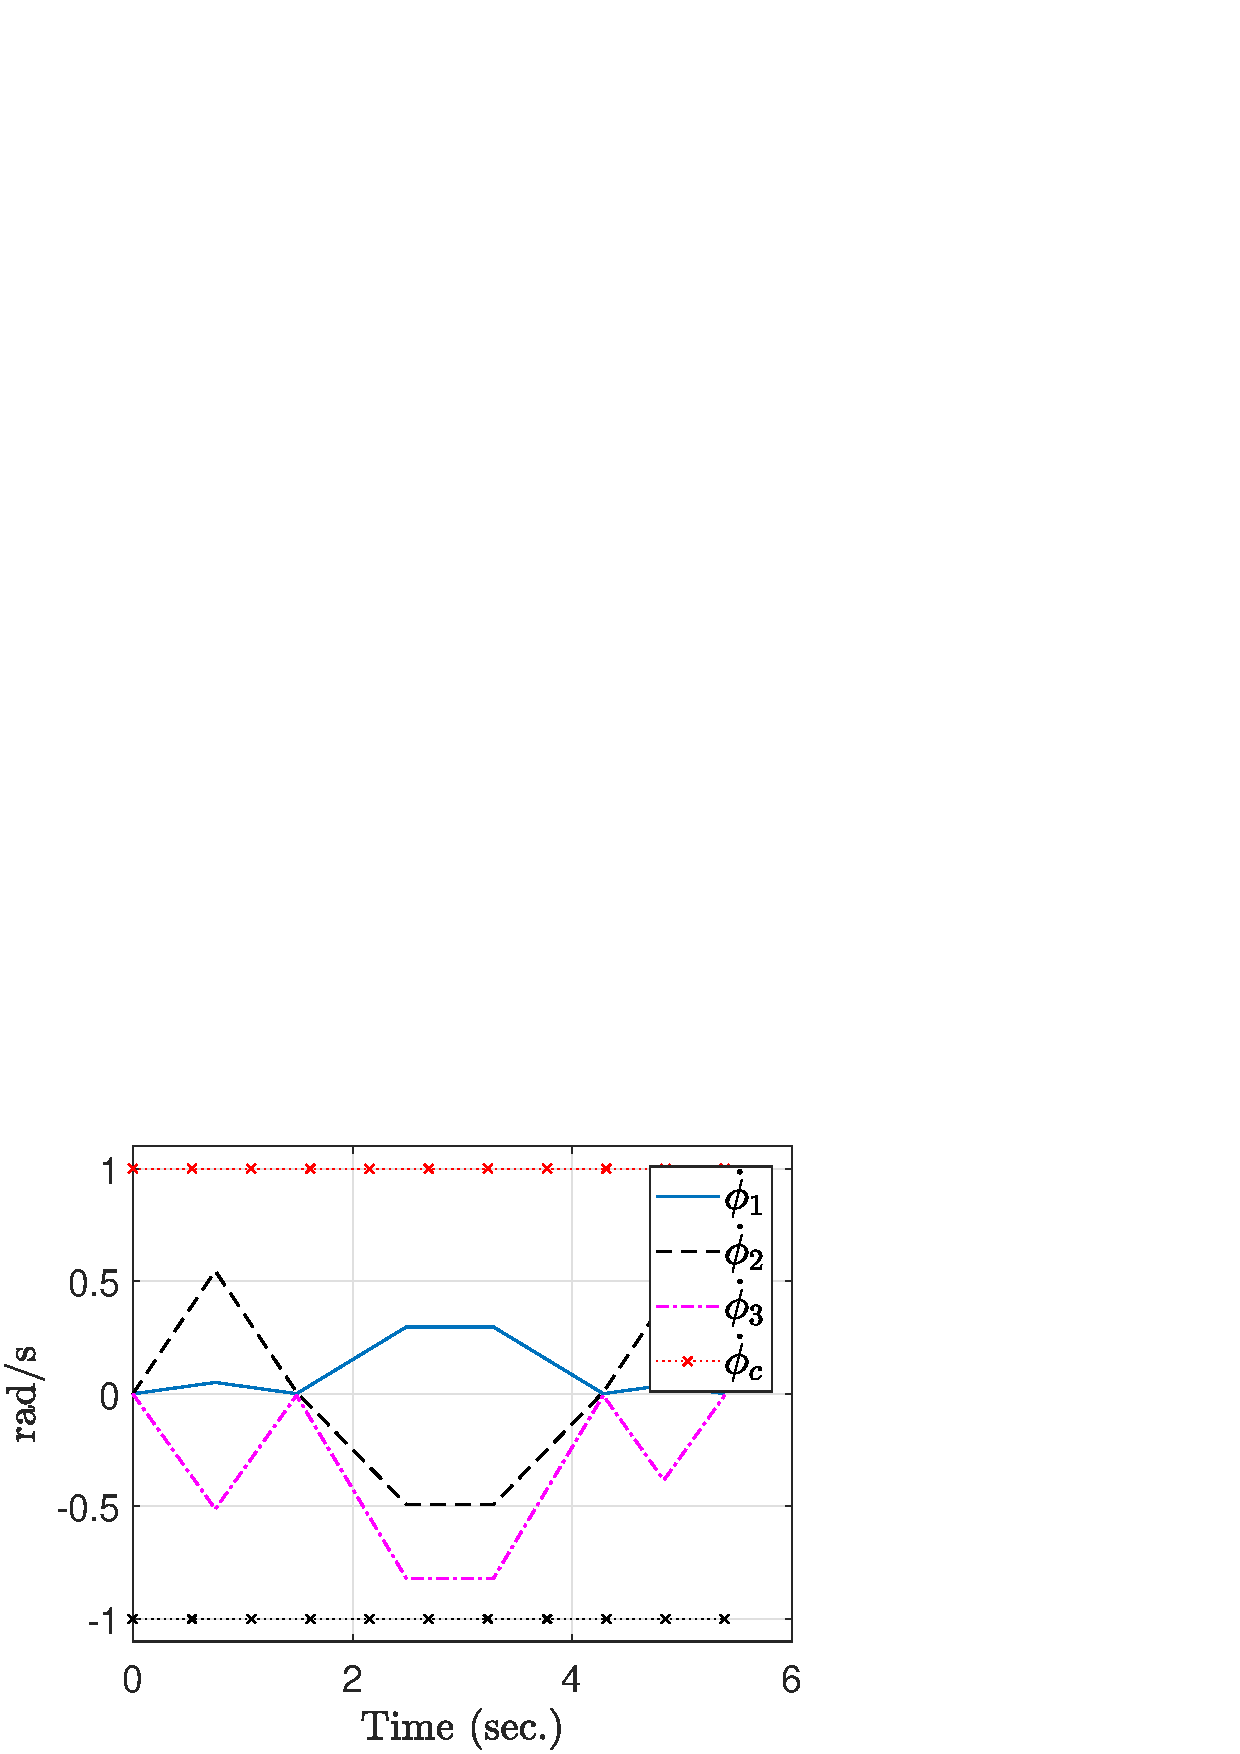
\includegraphics[width=3in]{figures/alphaNot0/ang_vel_phi_total.png}
			\caption{Angular Velocity when $\alpha>0$.}
			\label{fig:ang_vel_phi_total}
			\end{center}
		\end{figure}
	\columnbreak
		\begin{figure}[H]
%			\centering
			\begin{center}
				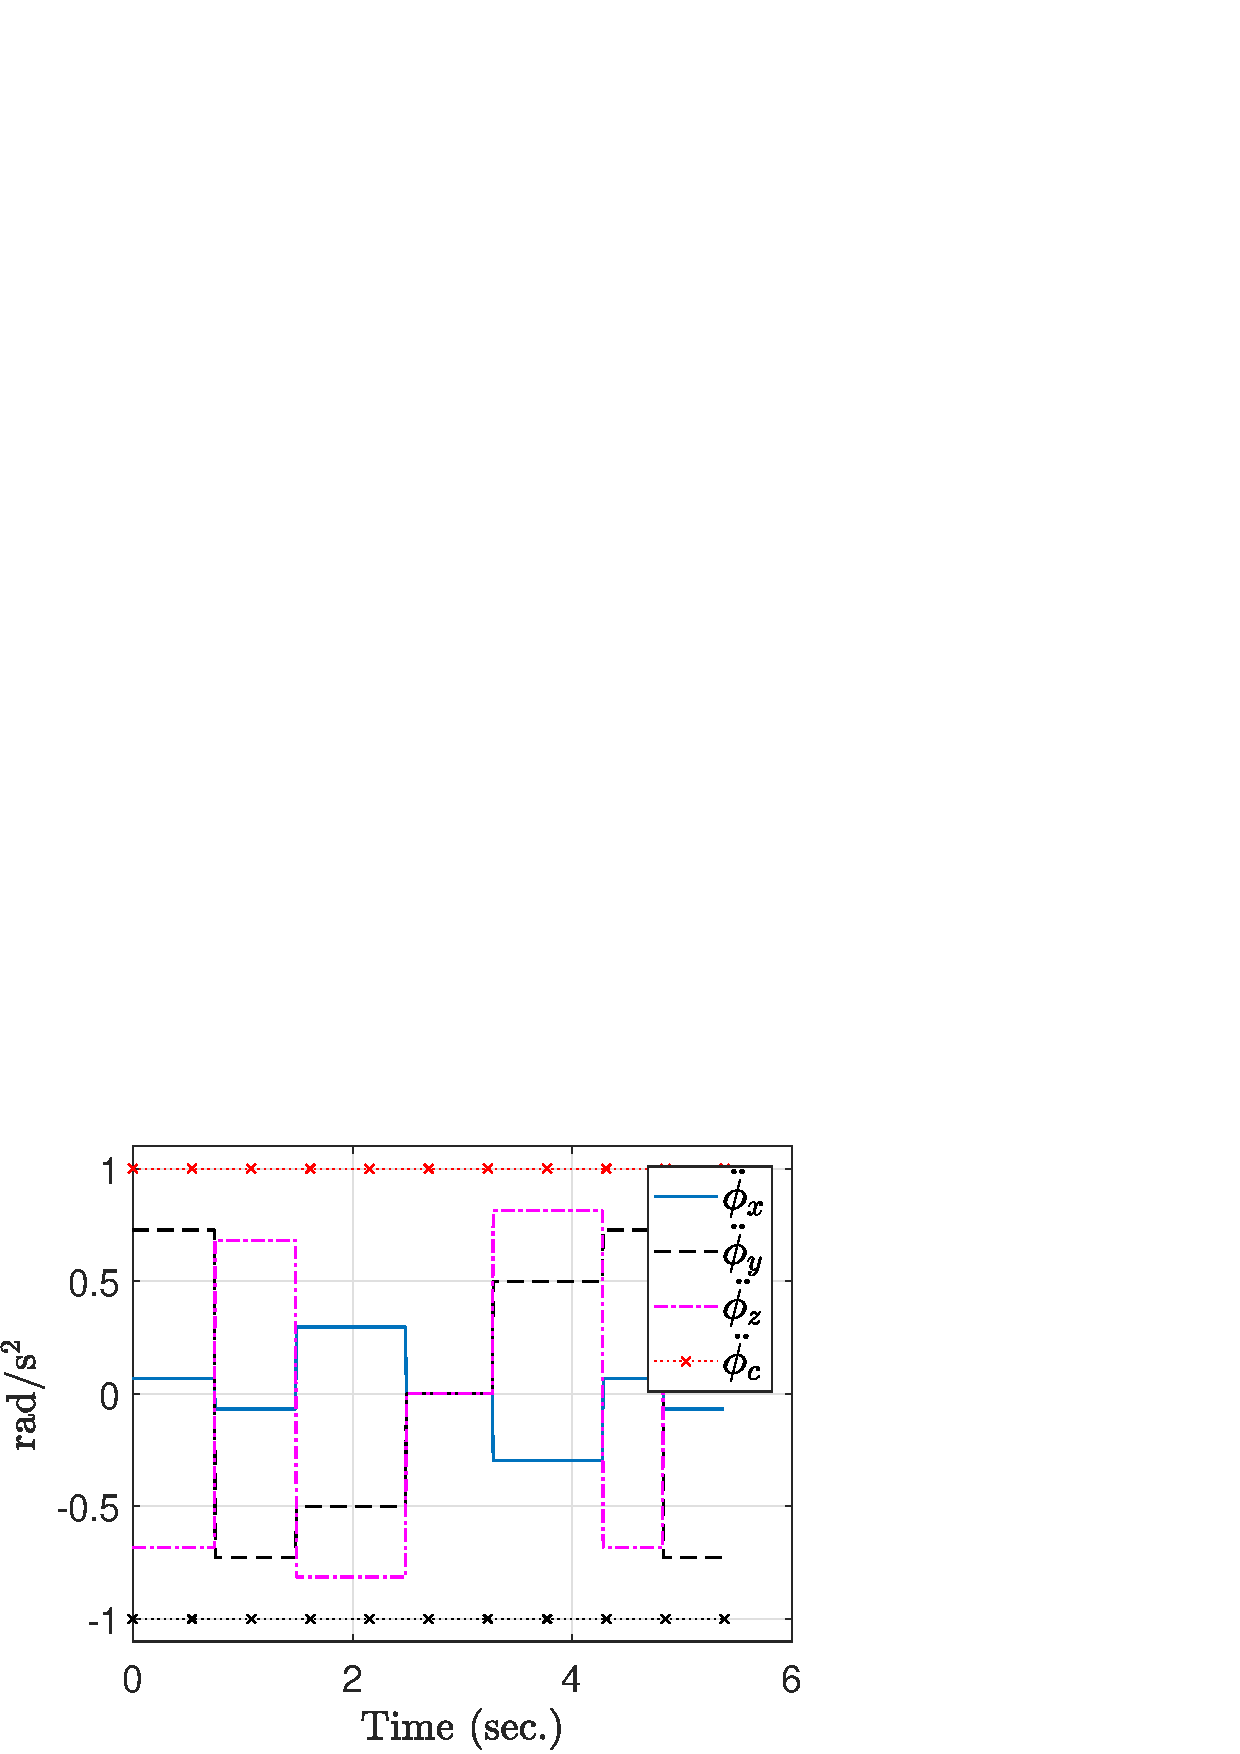
\includegraphics[width=3in]{figures/alphaNot0/ang_accel_total.png}
				\caption{Angular Acceleration when $\alpha>0$.}
				\label{fig:ang_accel_total}
			\end{center}
		\end{figure}
	\end{multicols}

Only the angular velocity and acceleration plots have constraints. In real life, the spacecraft's reaction wheels' ability to impart angular momentum is translated to a constraint in angular velocity, and the thrusters ability to impose torque translates to a constraint in angular acceleration. Therefore, there is no torque constraint plotted. 

Due to the high velocity and acceleration constraints, there is no coasting period for the $\phi_1$ and $\phi_3$ portions of the slew. However, there is a period of 0 angular acceleration constant angular velocity for $\phi_2$, which is reflected in the Figures \ref{fig:ang_vel_phi_total} and \ref{fig:ang_accel_total}. The attitude and torque profiles are shown in Figures \ref{fig:quats_phi_total} and \ref{fig:torque_total}. 
	
	\begin{multicols}{2}
		\begin{figure}[H]
			\begin{center}
			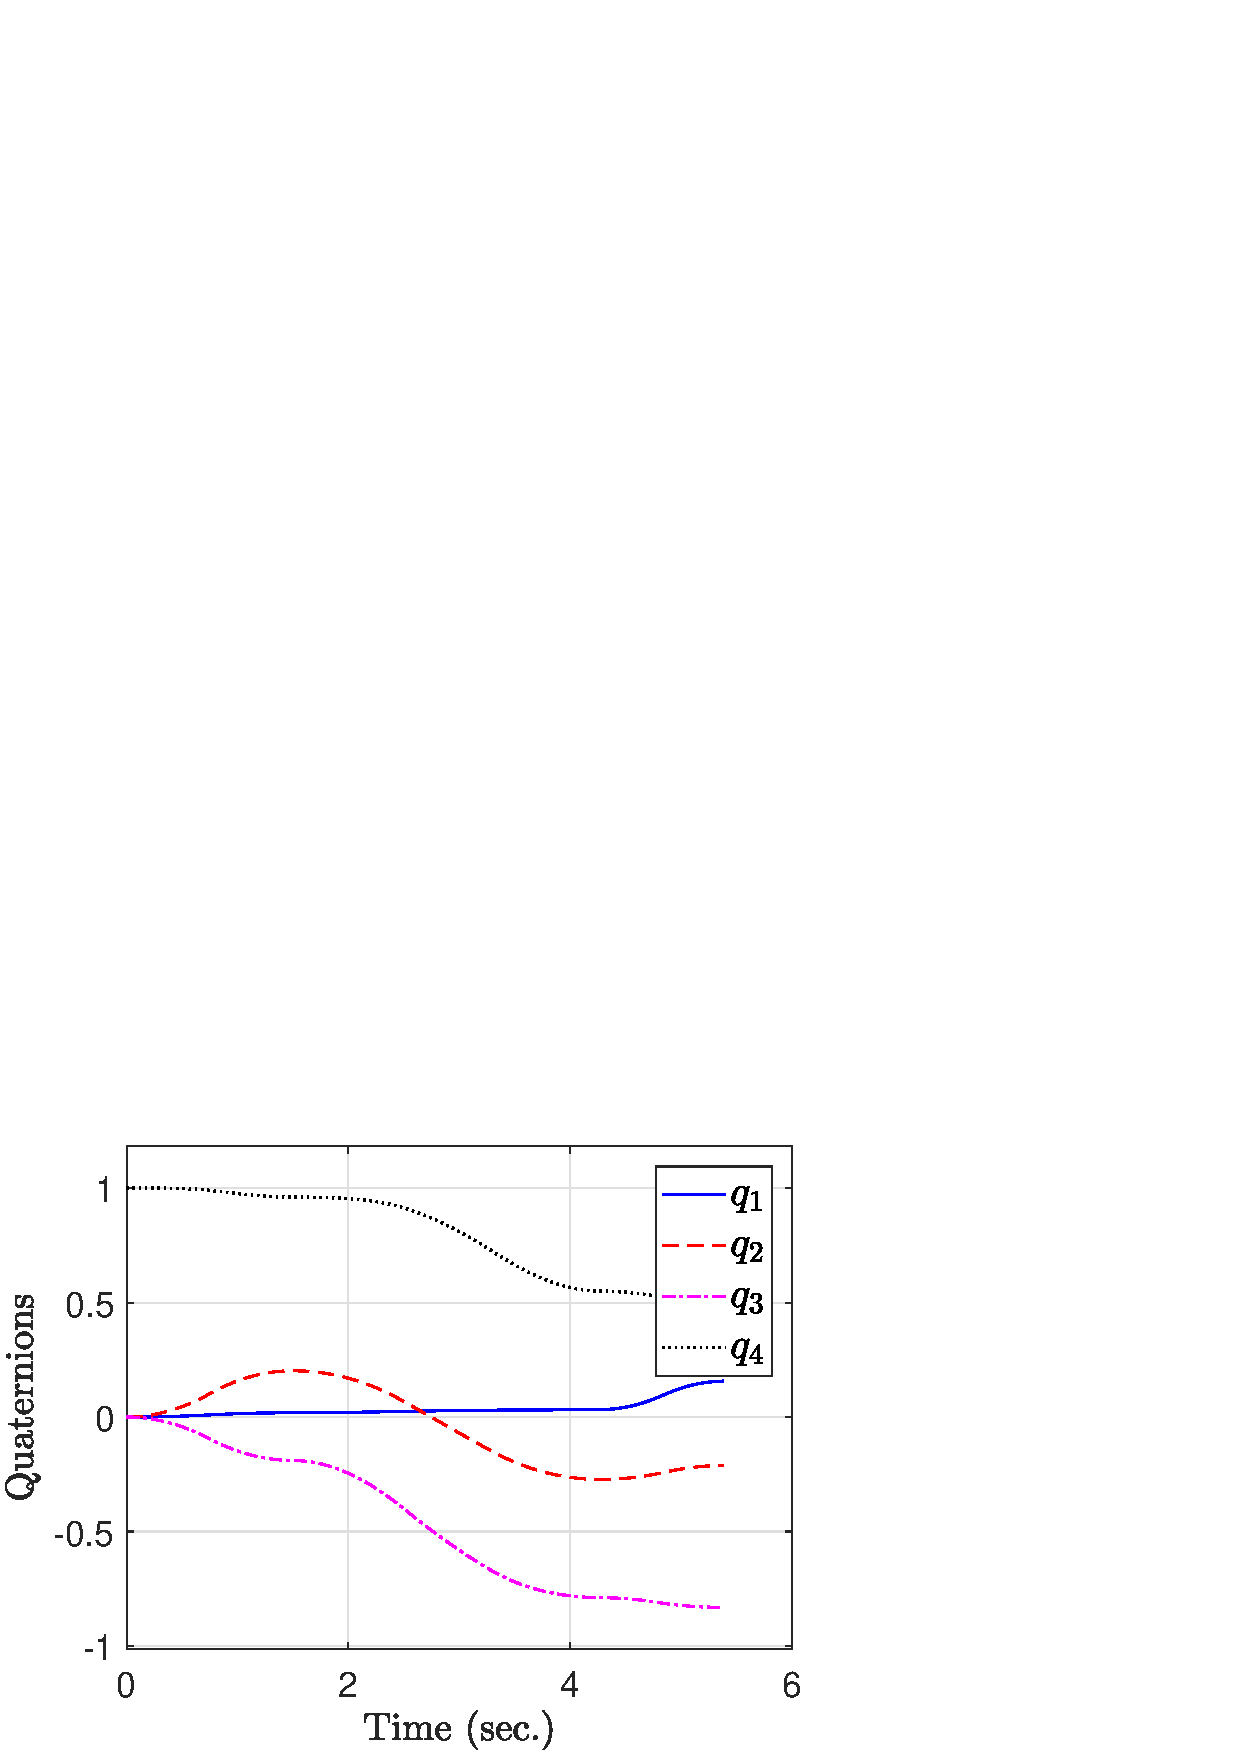
\includegraphics[width=3in]{figures/alphaNot0/quats_phi_total.png}
			\caption{Quaternions when $\alpha>0$.}
			\label{fig:quats_phi_total}
			\end{center}
		\end{figure}
	\columnbreak
		\begin{figure}[H]
			\begin{center}
			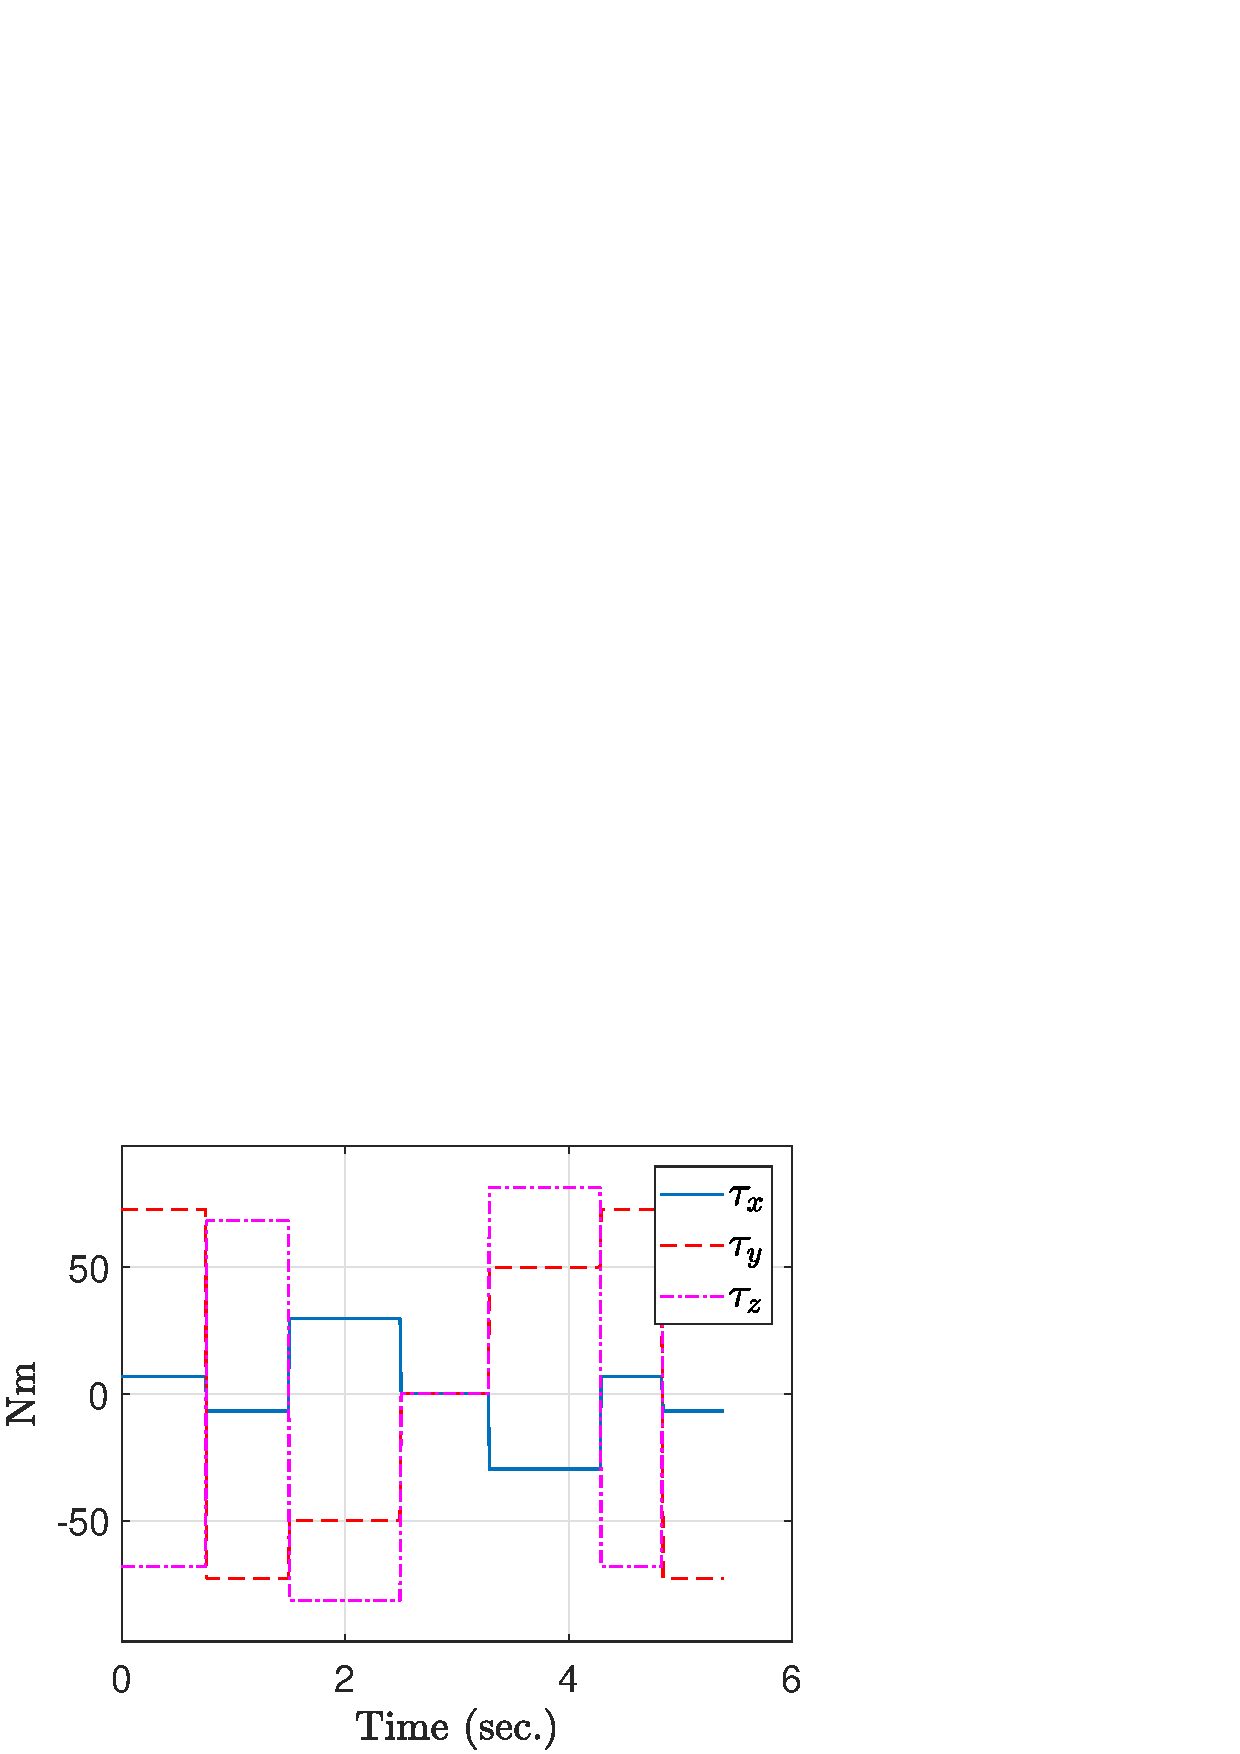
\includegraphics[width=3in]{figures/alphaNot0/torque_total.png}
			\end{center}
			\caption{Torque when $\alpha>0$.}
			\label{fig:torque_total}
		\end{figure}
	\end{multicols}
			
\subsection{Case II: $\alpha = 0$} 
			
For the case in which the sun vector lies directly on the slew plane, $\phi_2$ = 180 degrees. The initial, final, and sun positions in the inertial frame and the constraints are in Table \ref{tab:alpha0_PiPfS_AWmax}. 
			
			\begin{figure}[H]
			\begin{center}
				\includegraphics[width=4.75in]{figures/alpha0/phi1_phi2_phi3.png}
				\caption{Attitude Profile of the Entire Slew when $\alpha=0$.}
			\end{center}
			\label{fig:phi1_phi2_phi3_alpha0}
			\end{figure}	
		
The previous case, in which $\alpha > 0 $, had acceleration and velocity constraints of 1 rad/s$^2$ and 1 rad/s respectively, to demonstrate the if-else statements for switching times in case $\phi > \phi_t$. For this example, much more realistic constraints were imposed to reflect how the acceleration and velocity profiles would look like in real life. 
			
	\begin{multicols}{2}
		\begin{center}
			\begin{table}[H]
				\centering
				\caption{Initial, Final, and Sun Positions in Inertial Frame and Constraints (inputs)}
				\begin{tabular}{lc}
					\toprule
					\midrule
					Unit Vector & Comp \\
					\midrule
					$P_i$ & [0.65, -0.35, -0.67] \\
					$P_f$ & [-0.93, -0.25, 0.28] \\ 
					$S$ & [-0.20, -0.78, -0.59] \\
					\midrule
					\midrule
					Parameter & Constraint \\ 
					\midrule
					$\alpha_{max}$ & 0.02 $rad/s^2$ \\
					$\omega_{max}$ & 0.01 $rad/s$ \\ 
					\midrule
					\bottomrule
				\end{tabular}%
				\label{tab:alpha0_PiPfS_AWmax}%
			\end{table}
		\end{center}
	\columnbreak
		\begin{center}
			\begin{table}[H]
				\centering
				\caption{Slew Angles $\phi_1$, $\phi_2$, and $\phi_3$}
				\begin{tabular}{lc}
					\toprule
					\midrule
					$\phi$ & deg \\
					\midrule
					1 & 41.82 \\
					2 & 180.00 \\ 
					3 & 62.45 \\
					\midrule
					\bottomrule
				\end{tabular}%
				\label{tab:alpha0_phi_123}%
			\end{table}%
		\end{center}
	\end{multicols}

With smaller constraints, the simulation takes much longer to complete the slew maneuvers. Figures \ref{fig:ang_vel_phi_total_alpha0} and \ref{fig:torque_total_alpha0} show that the torque and acceleration applied are very short compared to the duration of the entire maneuver, in contrast to Figures \ref{fig:ang_accel_total} and \ref{fig:torque_total}. The spacecraft spends the majority of the time coasting at constant angular velocity, as seen in Figure \ref{fig:ang_accel_total_alpha0}. Though the initial and final points are further apart in the gyrostat unit sphere to begin with, the simulation takes an order of magnitude longer to complete at almost 500 seconds for $\alpha = 0$, as opposed to almost 5.5 seconds for $\alpha > 0$. The case shown here is much more realistic example that reflects real-world conditions. 
			
			% Columns: 
			\begin{multicols}{2}
				\begin{figure}[H]
					\begin{center}
						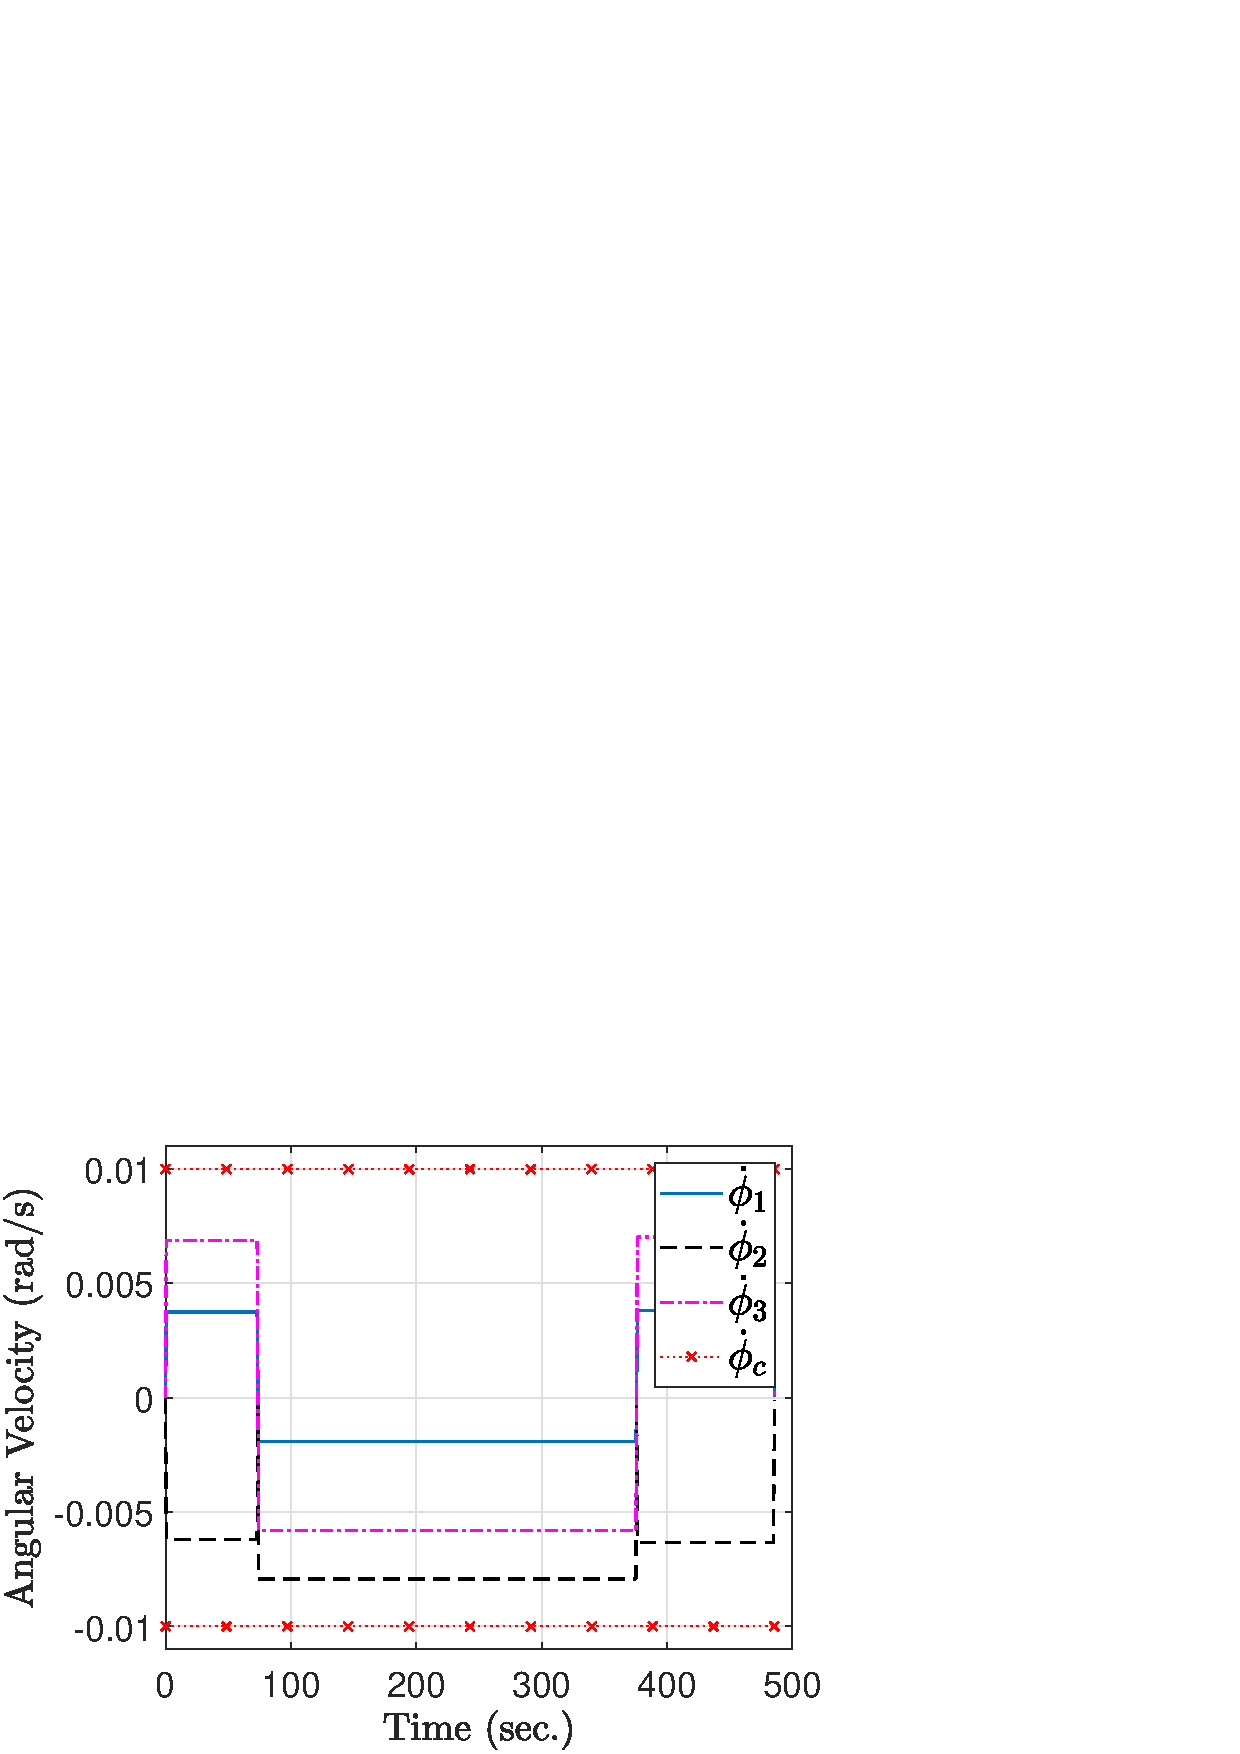
\includegraphics[width=3in]{figures/alpha0/ang_vel.png}
					\end{center}
					\caption{Angular Velocity when $\alpha=0$.}
					\label{fig:ang_vel_phi_total_alpha0}
				\end{figure}
				\columnbreak
				\begin{figure}[H]
					\begin{center}
						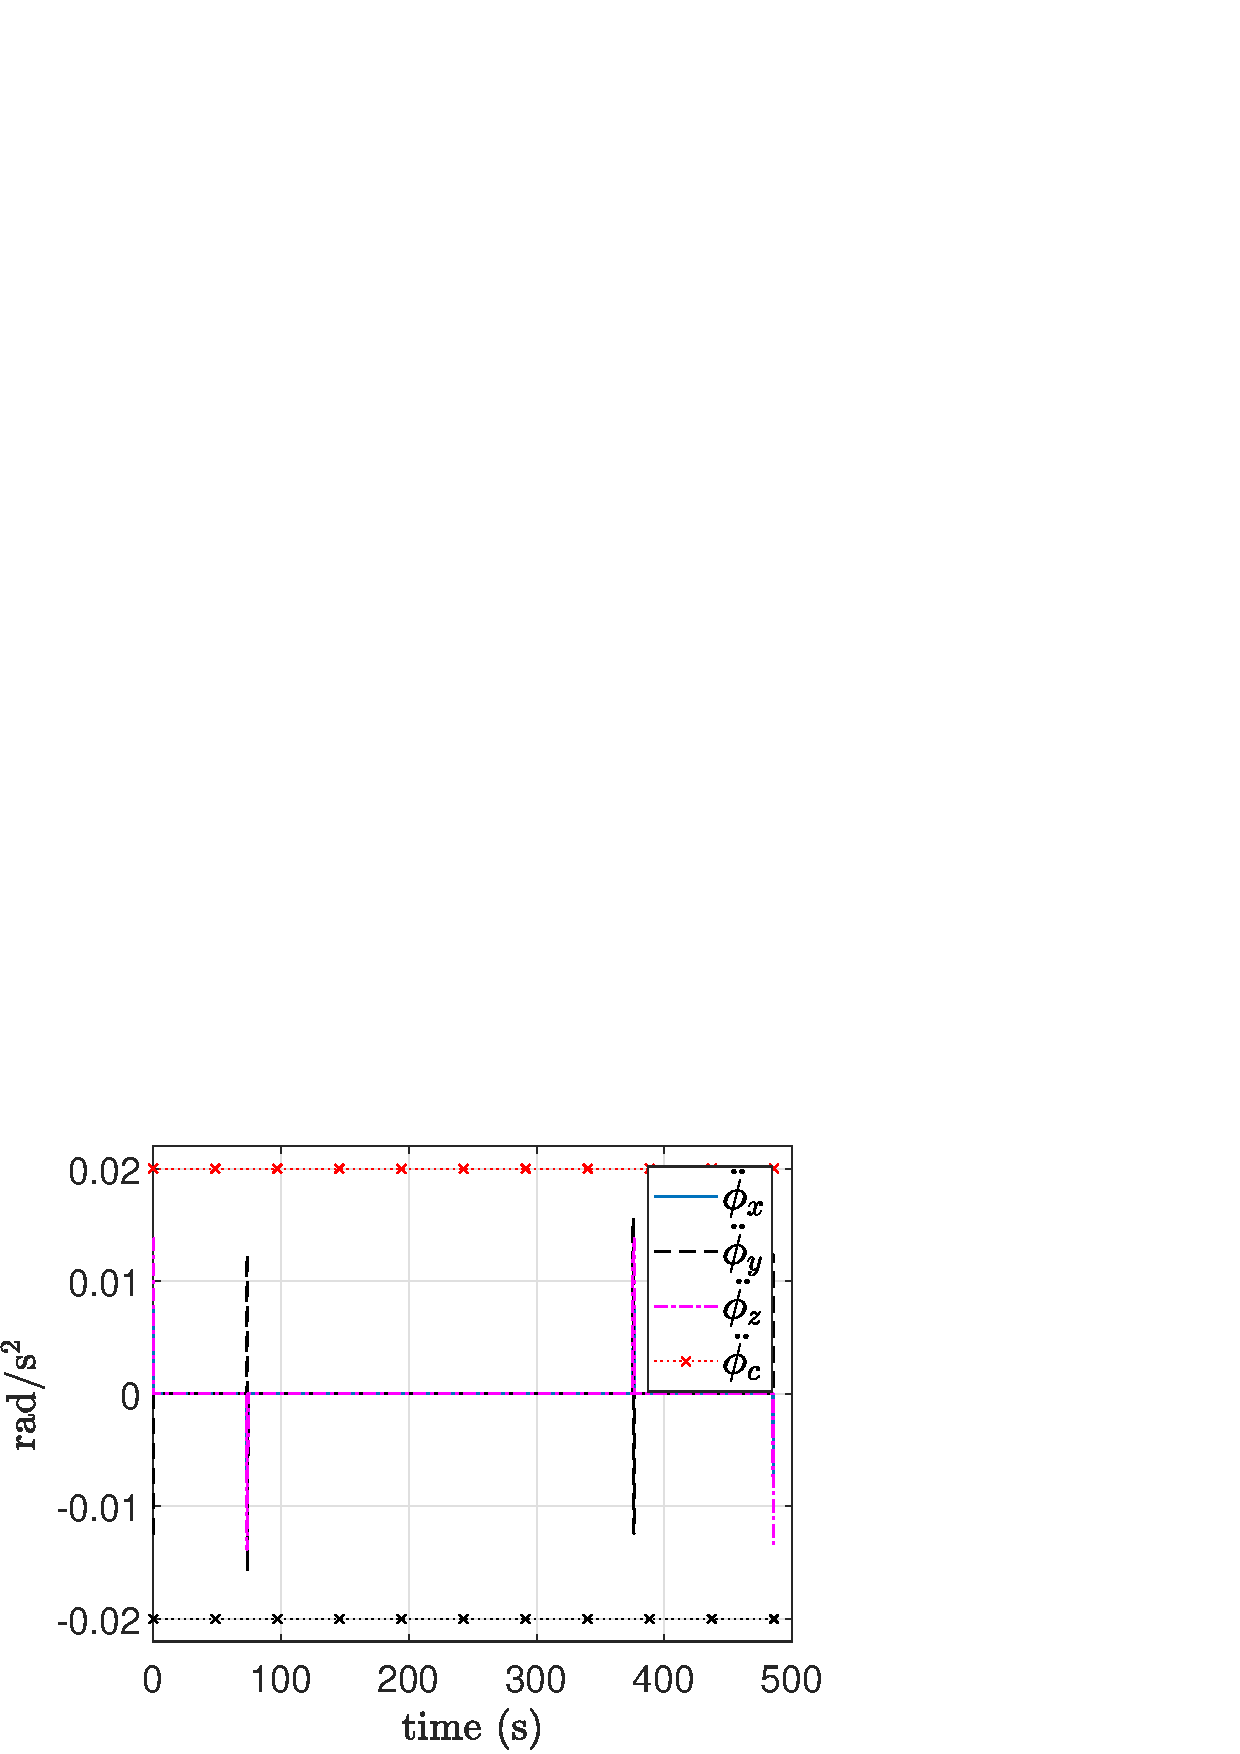
\includegraphics[width=3in]{figures/alpha0/ang_accel.png}
					\end{center}
					\caption{Angular Acceleration when $\alpha=0$.}
					\label{fig:ang_accel_total_alpha0}
				\end{figure}
			\end{multicols}
		
		\begin{multicols}{2}
			\begin{figure}[H]
				\begin{center}
					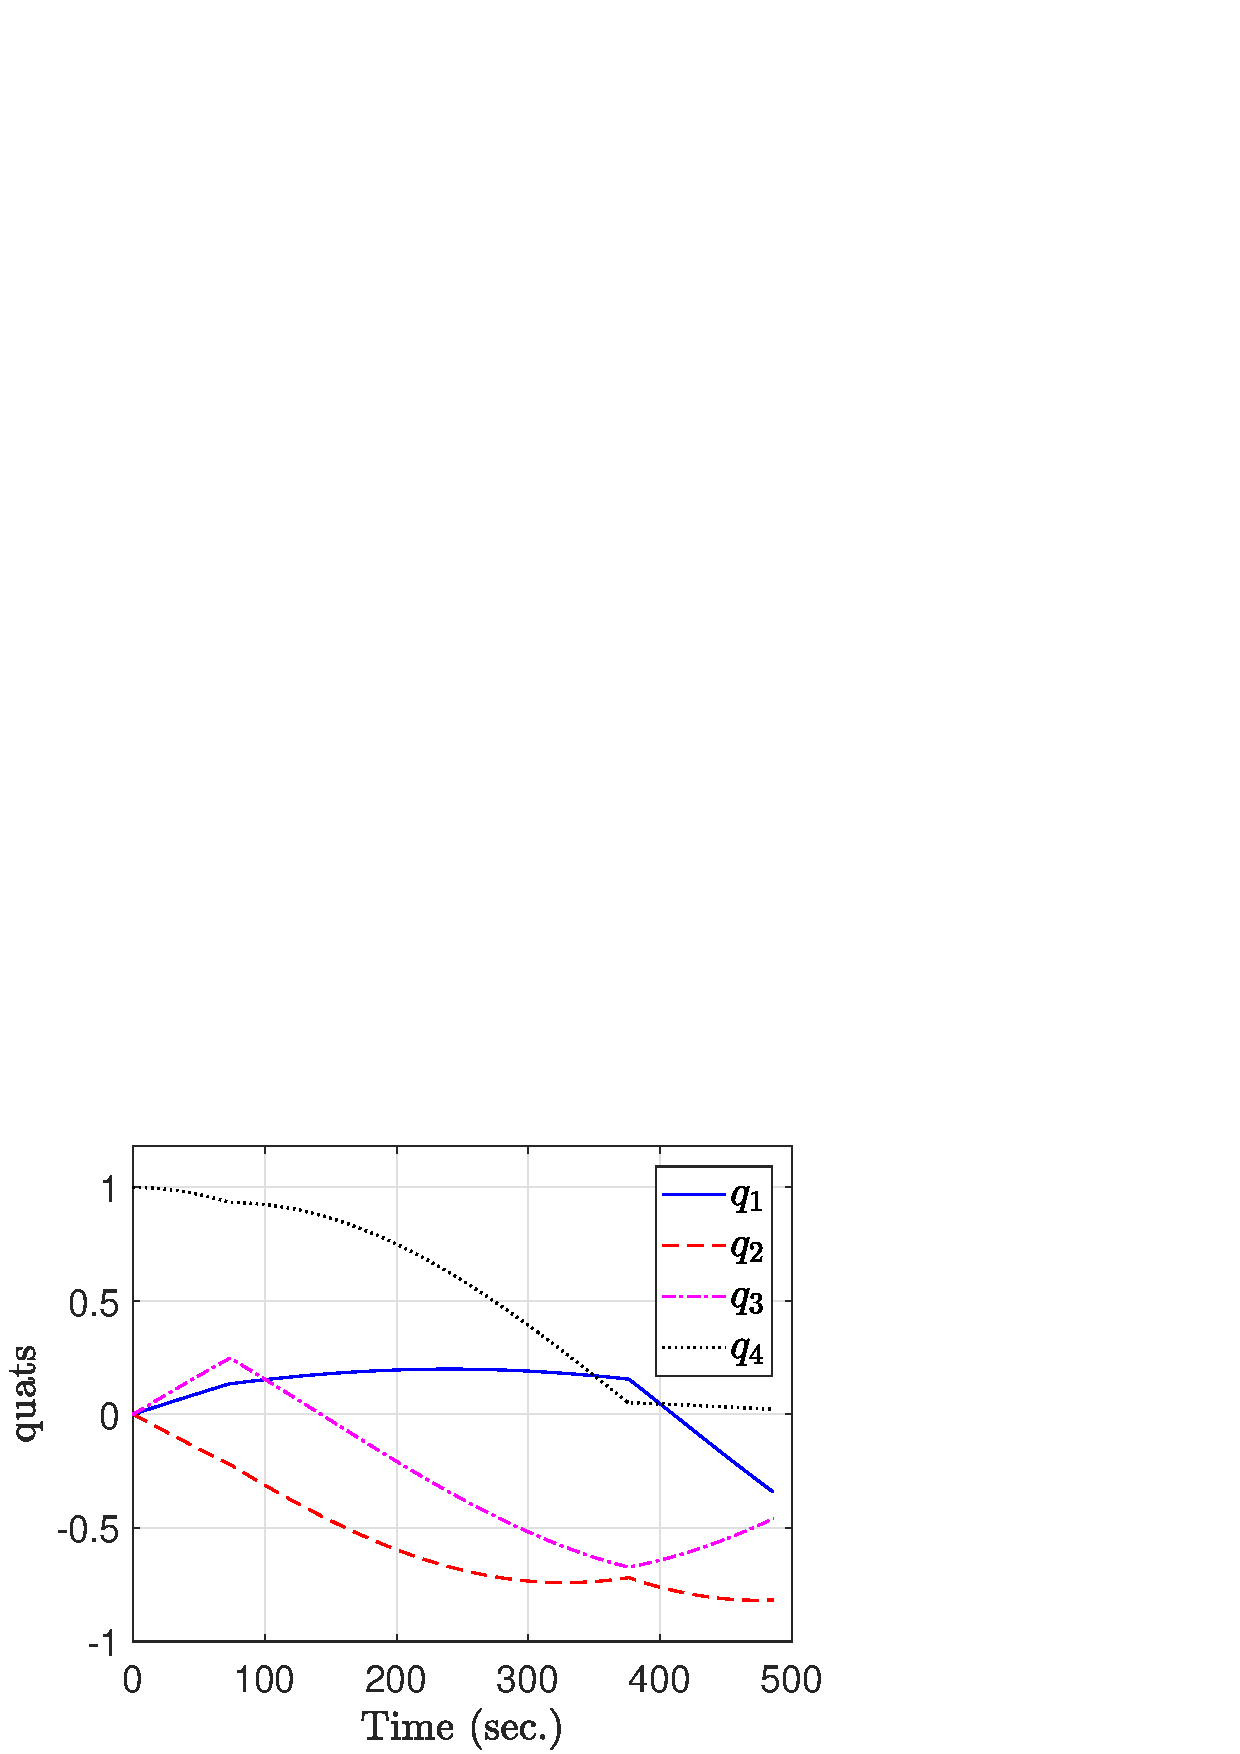
\includegraphics[width=3in]{figures/alpha0/quats.png}
				\end{center}
				\caption{Quaternions when $\alpha=0$.}
				\label{fig:quats_phi_total_alpha0}
			\end{figure}
			\columnbreak
			\begin{figure}[H]
				\begin{center}
					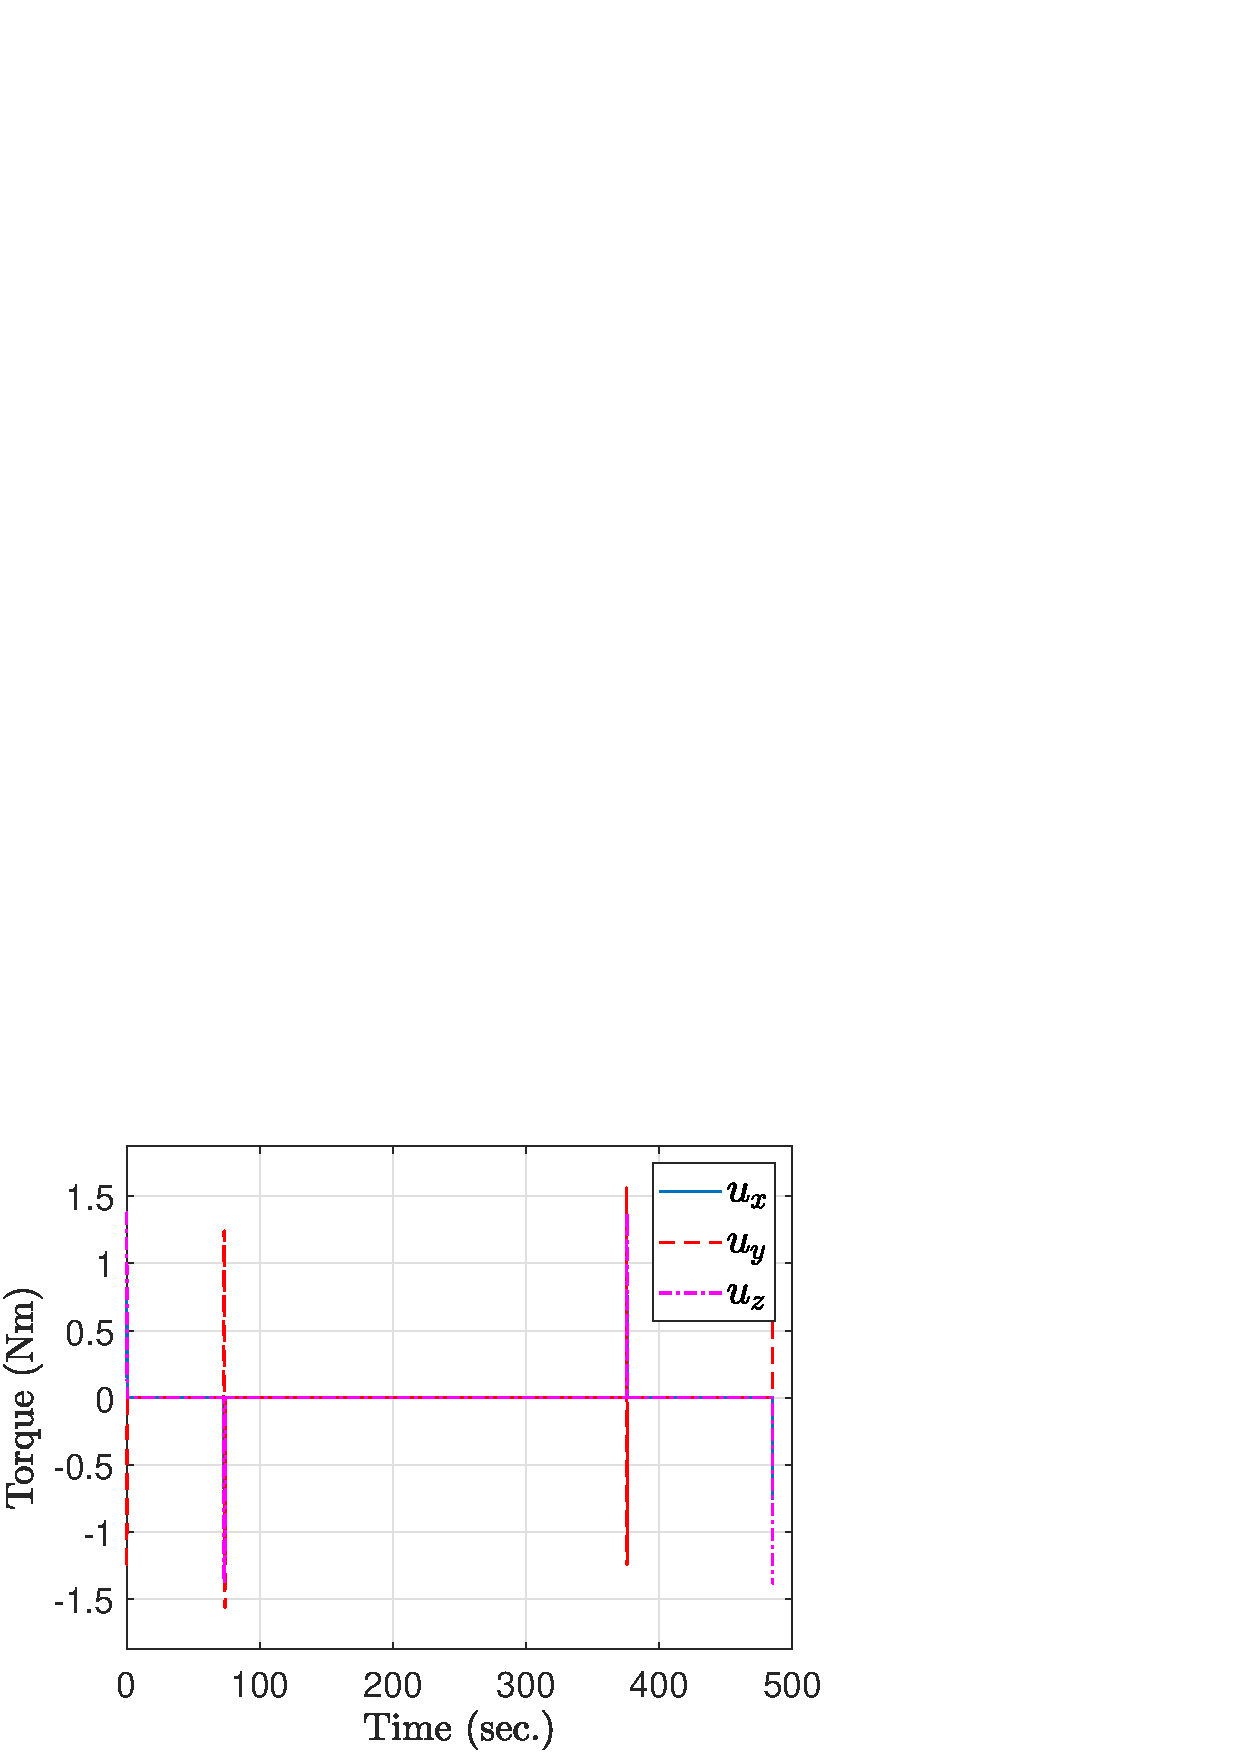
\includegraphics[width=3in]{figures/alpha0/torque.png}
				\end{center}
				\caption{Applied Torque when $\alpha=0$.}
				\label{fig:torque_total_alpha0}
			\end{figure}
		\end{multicols}
			
%%%%%%%%%%%%
	
\end{document}